%% The Appendices part is started with the command \appendix;
%% appendix sections are then done as normal sections
\newpage
\appendix
\section{Supplementary figures and tables}
\begin{figure}[htbp]
    \centering
    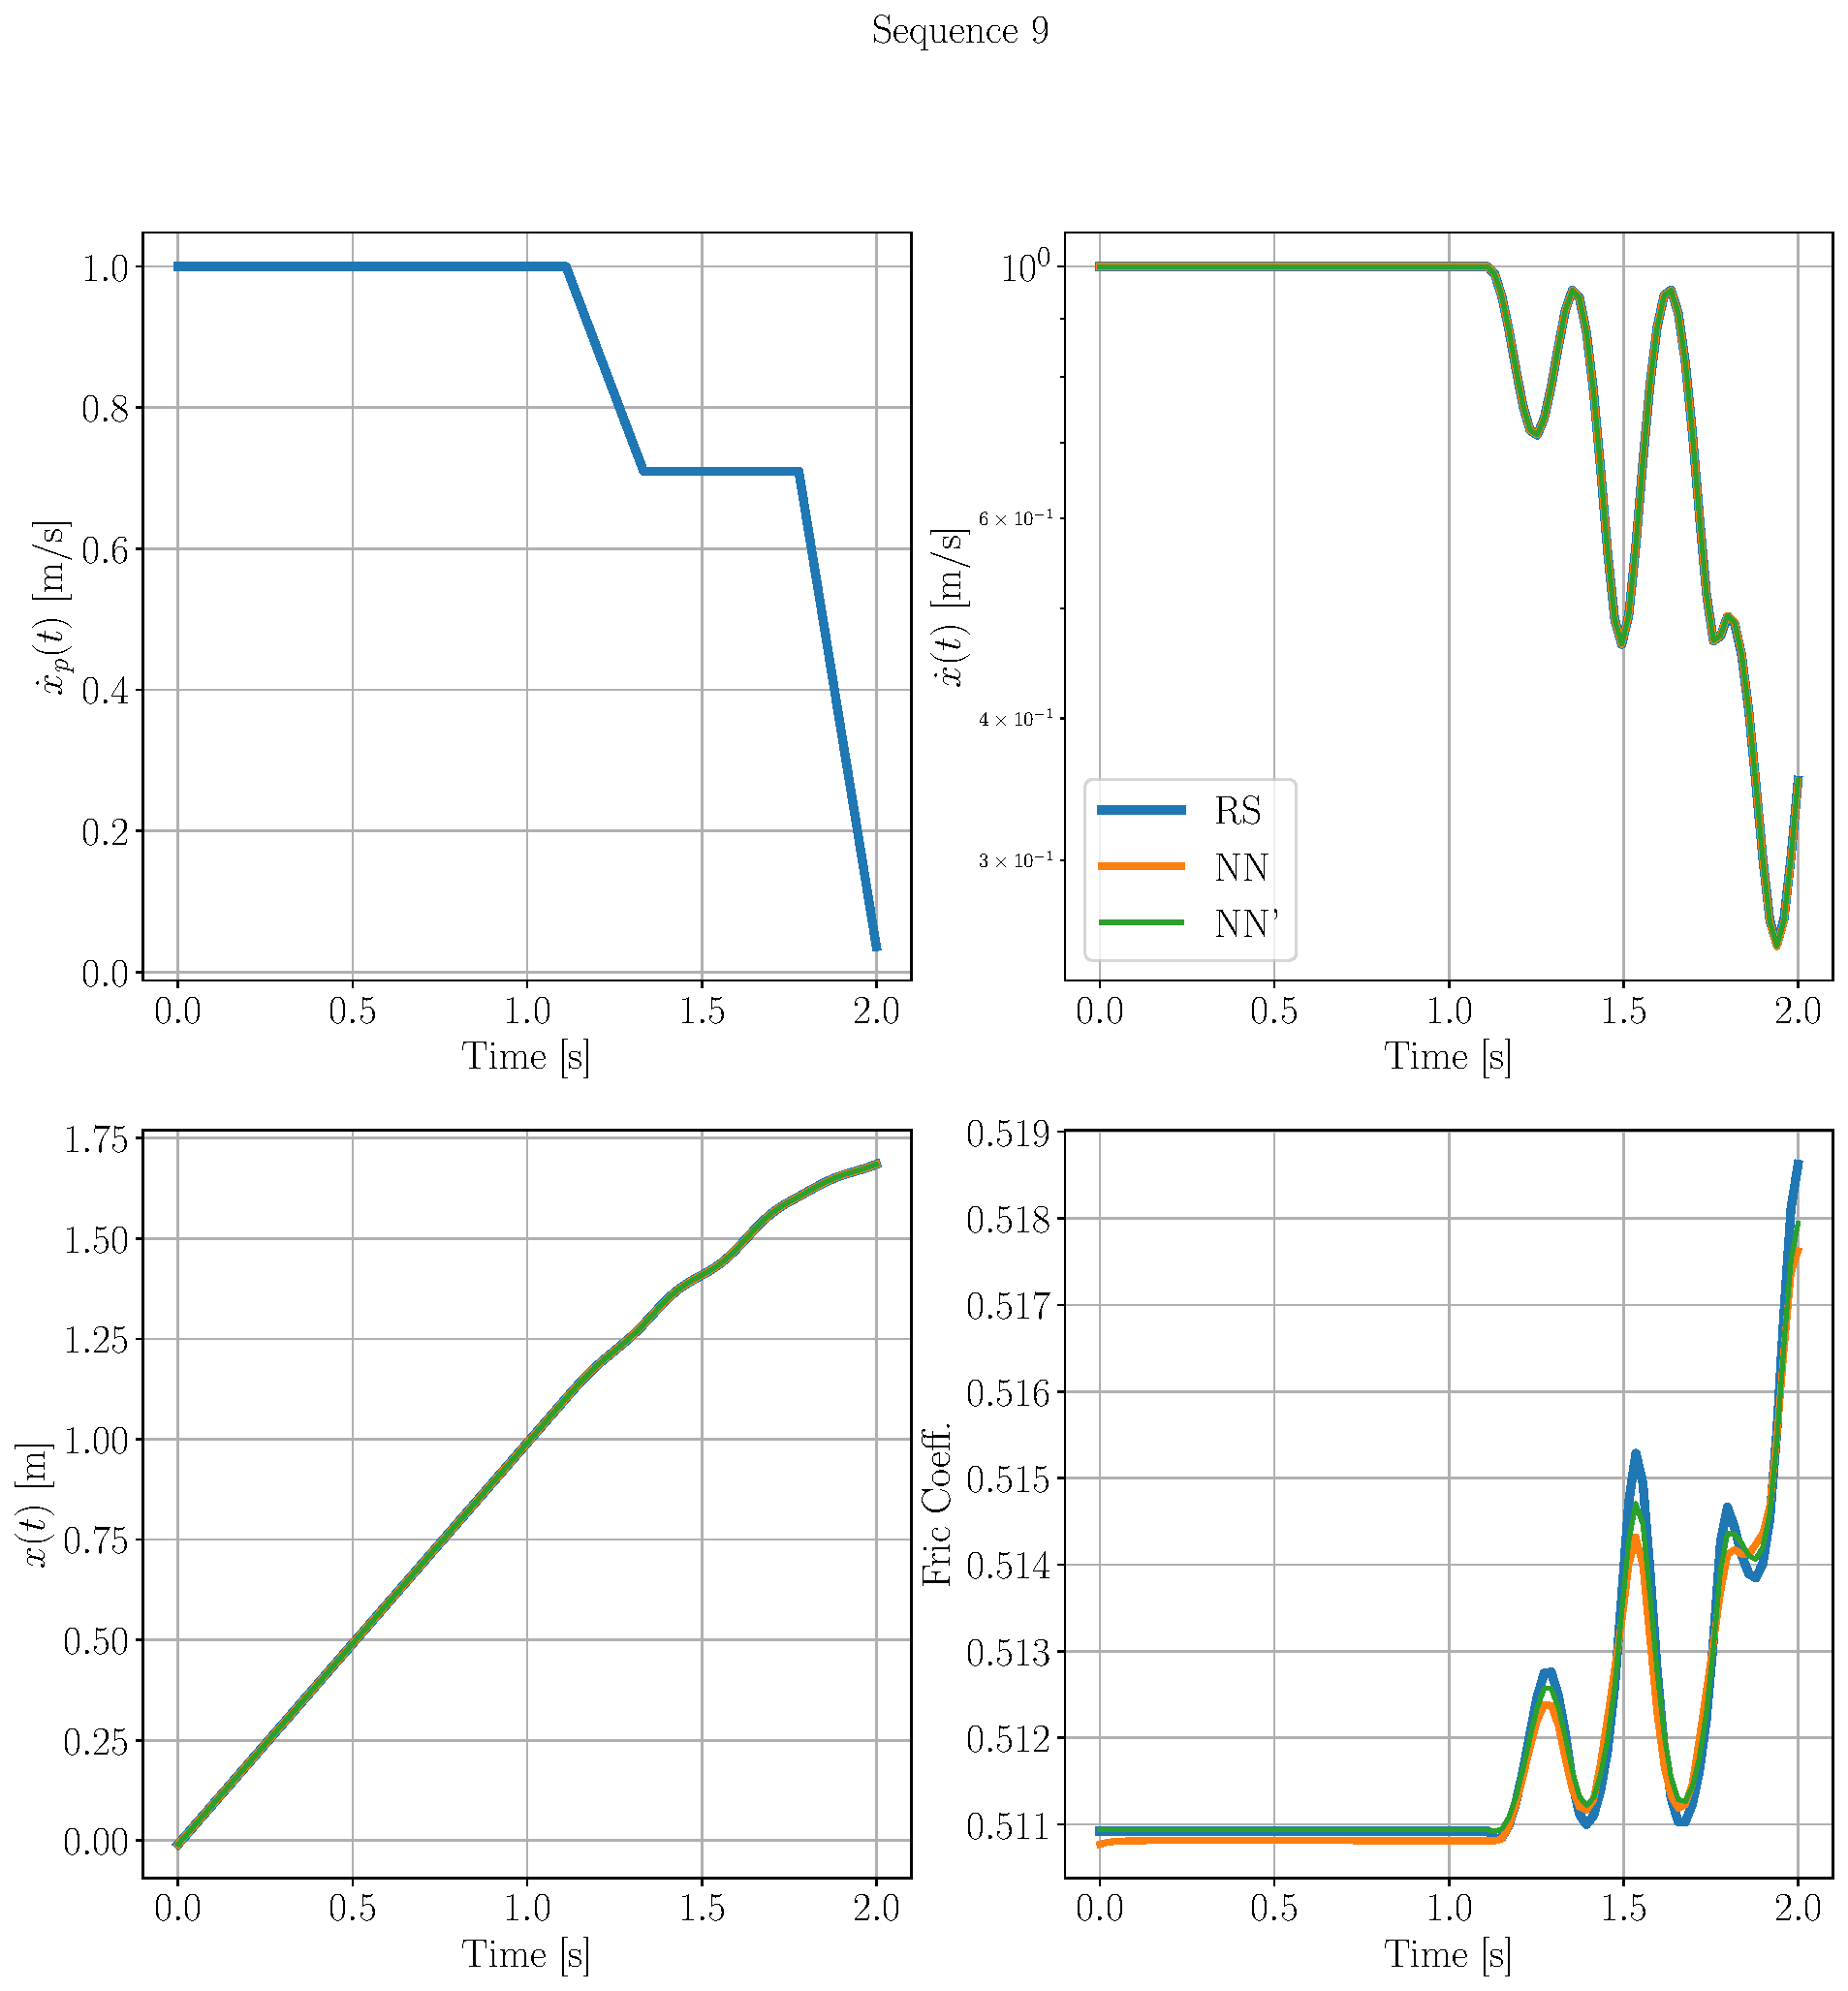
\includegraphics[width=0.9\textwidth]{figures/SS_seq9_0216_0521SS_combined_800.pdf}
    \caption{An example sequence of spring-slider solution with original rate-and-state friction, 
    NN potentials, 
    and NN potentials further trained on spring-slider sequences}
    \label{fig:SSseq9}
\end{figure}

\begin{table}[htbp]
    \centering
    \begin{tabular}{ccccccc}
        \hline
        $\Delta t$ [s] & $2^{-13.5}$ & $2^{-13.0}$ & $2^{-12.5}$ & $2^{-12.0}$ & $2^{-11.5}$ & $2^{-11.0}$ \\
        \hline
        NN, implicit & 5.993e-06 & 3.636e-06 & 4.807e-06 & 4.716e-06 & 6.282e-06 & 8.508e-06 \\
        NN, explicit & 6.130e-06 & 3.808e-06 & 4.786e-06 & 4.397e-06 & 5.968e-06 & 7.795e-06 \\
        RS, implicit & nan & nan & nan & nan & nan & nan \\
        RS, explicit & 7.321e-06 & 4.447e-06 & 5.267e-06 & 4.426e-06 & 6.464e-06 & 8.069e-06 \\
        \hline
    \end{tabular}
    \caption{Mean relative $L_2$ error in $\dot{x}(t)$ averaged over 77 sequences, 
    for NN, RS models with implicit, explicit solvers.}
    \label{tab:MeanL2ErrorSpringSliderRsVsNNRespective}
\end{table}

\begin{table}[htbp]
    \centering
    \begin{tabular}{cccccccc}
        \hline
        $\Delta t$ [s] & $2^{-13.5}$ & $2^{-13.0}$ & $2^{-12.5}$ & $2^{-12.0}$ & $2^{-11.5}$ & $2^{-11.0}$ \\
        \hline
        NN, implicit & 5.799e-06 & 5.390e-06 & 5.575e-06 & 7.069e-06 & 6.384e-06 & 1.033e-05 \\
        NN, explicit & 6.241e-06 & 5.766e-06 & 5.844e-06 & 6.887e-06 & 6.572e-06 & 9.639e-06 \\
        RS, implicit & nan & nan & nan & nan & nan & nan \\
        RS, explicit & 9.601e-06 & 6.886e-06 & 5.541e-06 & 5.597e-06 & 6.845e-06 & 1.017e-05 \\
        \hline
    \end{tabular}
    \caption{Standard deviation of relative $L_2$ error in $\dot{x}(t)$ over 77 sequences, 
    for NN, RS models with implicit, explicit solvers.}
    \label{tab:StdL2ErrorSpringSliderRsVsNNRespective}
\end{table}